
	
		\begin{figure*}
			\center
			% \subcaphangtrue
			\begin{subfigure}[t]{0.33\textwidth}
				\centerline{
					% GNUPLOT: LaTeX picture with Postscript
\begingroup
  \makeatletter
  \providecommand\color[2][]{%
    \GenericError{(gnuplot) \space\space\space\@spaces}{%
      Package color not loaded in conjunction with
      terminal option `colourtext'%
    }{See the gnuplot documentation for explanation.%
    }{Either use 'blacktext' in gnuplot or load the package
      color.sty in LaTeX.}%
    \renewcommand\color[2][]{}%
  }%
  \providecommand\includegraphics[2][]{%
    \GenericError{(gnuplot) \space\space\space\@spaces}{%
      Package graphicx or graphics not loaded%
    }{See the gnuplot documentation for explanation.%
    }{The gnuplot epslatex terminal needs graphicx.sty or graphics.sty.}%
    \renewcommand\includegraphics[2][]{}%
  }%
  \providecommand\rotatebox[2]{#2}%
  \@ifundefined{ifGPcolor}{%
    \newif\ifGPcolor
    \GPcolorfalse
  }{}%
  \@ifundefined{ifGPblacktext}{%
    \newif\ifGPblacktext
    \GPblacktexttrue
  }{}%
  % define a \g@addto@macro without @ in the name:
  \let\gplgaddtomacro\g@addto@macro
  % define empty templates for all commands taking text:
  \gdef\gplbacktext{}%
  \gdef\gplfronttext{}%
  \makeatother
  \ifGPblacktext
    % no textcolor at all
    \def\colorrgb#1{}%
    \def\colorgray#1{}%
  \else
    % gray or color?
    \ifGPcolor
      \def\colorrgb#1{\color[rgb]{#1}}%
      \def\colorgray#1{\color[gray]{#1}}%
      \expandafter\def\csname LTw\endcsname{\color{white}}%
      \expandafter\def\csname LTb\endcsname{\color{black}}%
      \expandafter\def\csname LTa\endcsname{\color{black}}%
      \expandafter\def\csname LT0\endcsname{\color[rgb]{1,0,0}}%
      \expandafter\def\csname LT1\endcsname{\color[rgb]{0,1,0}}%
      \expandafter\def\csname LT2\endcsname{\color[rgb]{0,0,1}}%
      \expandafter\def\csname LT3\endcsname{\color[rgb]{1,0,1}}%
      \expandafter\def\csname LT4\endcsname{\color[rgb]{0,1,1}}%
      \expandafter\def\csname LT5\endcsname{\color[rgb]{1,1,0}}%
      \expandafter\def\csname LT6\endcsname{\color[rgb]{0,0,0}}%
      \expandafter\def\csname LT7\endcsname{\color[rgb]{1,0.3,0}}%
      \expandafter\def\csname LT8\endcsname{\color[rgb]{0.5,0.5,0.5}}%
    \else
      % gray
      \def\colorrgb#1{\color{black}}%
      \def\colorgray#1{\color[gray]{#1}}%
      \expandafter\def\csname LTw\endcsname{\color{white}}%
      \expandafter\def\csname LTb\endcsname{\color{black}}%
      \expandafter\def\csname LTa\endcsname{\color{black}}%
      \expandafter\def\csname LT0\endcsname{\color{black}}%
      \expandafter\def\csname LT1\endcsname{\color{black}}%
      \expandafter\def\csname LT2\endcsname{\color{black}}%
      \expandafter\def\csname LT3\endcsname{\color{black}}%
      \expandafter\def\csname LT4\endcsname{\color{black}}%
      \expandafter\def\csname LT5\endcsname{\color{black}}%
      \expandafter\def\csname LT6\endcsname{\color{black}}%
      \expandafter\def\csname LT7\endcsname{\color{black}}%
      \expandafter\def\csname LT8\endcsname{\color{black}}%
    \fi
  \fi
  \setlength{\unitlength}{0.0500bp}%
  \begin{picture}(3968.00,2834.00)%
    \gplgaddtomacro\gplbacktext{%
      \csname LTb\endcsname%
      \put(952,634){\makebox(0,0)[r]{\strut{} 0}}%
      \csname LTb\endcsname%
      \put(952,1021){\makebox(0,0)[r]{\strut{} 2}}%
      \csname LTb\endcsname%
      \put(952,1408){\makebox(0,0)[r]{\strut{} 4}}%
      \csname LTb\endcsname%
      \put(952,1795){\makebox(0,0)[r]{\strut{} 6}}%
      \csname LTb\endcsname%
      \put(952,2182){\makebox(0,0)[r]{\strut{} 8}}%
      \csname LTb\endcsname%
      \put(952,2569){\makebox(0,0)[r]{\strut{} 10}}%
      \csname LTb\endcsname%
      \put(1278,220){\makebox(0,0){\strut{} 0}}%
      \csname LTb\endcsname%
      \put(1665,220){\makebox(0,0){\strut{} 2}}%
      \csname LTb\endcsname%
      \put(2052,220){\makebox(0,0){\strut{} 4}}%
      \csname LTb\endcsname%
      \put(2439,220){\makebox(0,0){\strut{} 6}}%
      \csname LTb\endcsname%
      \put(2826,220){\makebox(0,0){\strut{} 8}}%
      \csname LTb\endcsname%
      \put(3213,220){\makebox(0,0){\strut{} 10}}%
    }%
    \gplgaddtomacro\gplfronttext{%
      \csname LTb\endcsname%
      \put(1403,2250){\makebox(0,0)[l]{\strut{}$P^\m{(SOC)}$}}%
    }%
    \gplbacktext
    \put(0,0){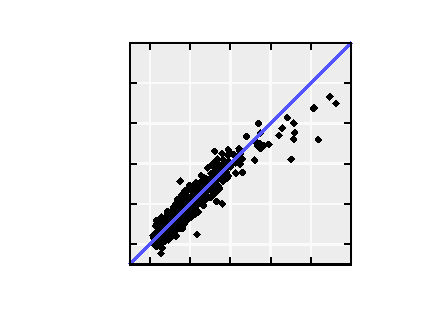
\includegraphics{gp/ms-sa-soc-corr}}%
    \gplfronttext
  \end{picture}%
\endgroup

				}
				\caption{\parbox[t]{0.45\textwidth}{
					$\hat{p}^{(\m{SOC})} \sim p^{(\m{SOC})}$ \smallskip \\
					$(R^2)^{(\m{SOC})} = 0.871$
					}}
			\end{subfigure}
			\begin{subfigure}[t]{0.33\textwidth}
				\centerline{
					% GNUPLOT: LaTeX picture with Postscript
\begingroup
  \makeatletter
  \providecommand\color[2][]{%
    \GenericError{(gnuplot) \space\space\space\@spaces}{%
      Package color not loaded in conjunction with
      terminal option `colourtext'%
    }{See the gnuplot documentation for explanation.%
    }{Either use 'blacktext' in gnuplot or load the package
      color.sty in LaTeX.}%
    \renewcommand\color[2][]{}%
  }%
  \providecommand\includegraphics[2][]{%
    \GenericError{(gnuplot) \space\space\space\@spaces}{%
      Package graphicx or graphics not loaded%
    }{See the gnuplot documentation for explanation.%
    }{The gnuplot epslatex terminal needs graphicx.sty or graphics.sty.}%
    \renewcommand\includegraphics[2][]{}%
  }%
  \providecommand\rotatebox[2]{#2}%
  \@ifundefined{ifGPcolor}{%
    \newif\ifGPcolor
    \GPcolorfalse
  }{}%
  \@ifundefined{ifGPblacktext}{%
    \newif\ifGPblacktext
    \GPblacktexttrue
  }{}%
  % define a \g@addto@macro without @ in the name:
  \let\gplgaddtomacro\g@addto@macro
  % define empty templates for all commands taking text:
  \gdef\gplbacktext{}%
  \gdef\gplfronttext{}%
  \makeatother
  \ifGPblacktext
    % no textcolor at all
    \def\colorrgb#1{}%
    \def\colorgray#1{}%
  \else
    % gray or color?
    \ifGPcolor
      \def\colorrgb#1{\color[rgb]{#1}}%
      \def\colorgray#1{\color[gray]{#1}}%
      \expandafter\def\csname LTw\endcsname{\color{white}}%
      \expandafter\def\csname LTb\endcsname{\color{black}}%
      \expandafter\def\csname LTa\endcsname{\color{black}}%
      \expandafter\def\csname LT0\endcsname{\color[rgb]{1,0,0}}%
      \expandafter\def\csname LT1\endcsname{\color[rgb]{0,1,0}}%
      \expandafter\def\csname LT2\endcsname{\color[rgb]{0,0,1}}%
      \expandafter\def\csname LT3\endcsname{\color[rgb]{1,0,1}}%
      \expandafter\def\csname LT4\endcsname{\color[rgb]{0,1,1}}%
      \expandafter\def\csname LT5\endcsname{\color[rgb]{1,1,0}}%
      \expandafter\def\csname LT6\endcsname{\color[rgb]{0,0,0}}%
      \expandafter\def\csname LT7\endcsname{\color[rgb]{1,0.3,0}}%
      \expandafter\def\csname LT8\endcsname{\color[rgb]{0.5,0.5,0.5}}%
    \else
      % gray
      \def\colorrgb#1{\color{black}}%
      \def\colorgray#1{\color[gray]{#1}}%
      \expandafter\def\csname LTw\endcsname{\color{white}}%
      \expandafter\def\csname LTb\endcsname{\color{black}}%
      \expandafter\def\csname LTa\endcsname{\color{black}}%
      \expandafter\def\csname LT0\endcsname{\color{black}}%
      \expandafter\def\csname LT1\endcsname{\color{black}}%
      \expandafter\def\csname LT2\endcsname{\color{black}}%
      \expandafter\def\csname LT3\endcsname{\color{black}}%
      \expandafter\def\csname LT4\endcsname{\color{black}}%
      \expandafter\def\csname LT5\endcsname{\color{black}}%
      \expandafter\def\csname LT6\endcsname{\color{black}}%
      \expandafter\def\csname LT7\endcsname{\color{black}}%
      \expandafter\def\csname LT8\endcsname{\color{black}}%
    \fi
  \fi
  \setlength{\unitlength}{0.0500bp}%
  \begin{picture}(3968.00,2834.00)%
    \gplgaddtomacro\gplbacktext{%
      \csname LTb\endcsname%
      \put(1018,677){\makebox(0,0)[r]{\strut{} 0}}%
      \csname LTb\endcsname%
      \put(1018,1150){\makebox(0,0)[r]{\strut{} 0.2}}%
      \csname LTb\endcsname%
      \put(1018,1623){\makebox(0,0)[r]{\strut{} 0.4}}%
      \csname LTb\endcsname%
      \put(1018,2096){\makebox(0,0)[r]{\strut{} 0.6}}%
      \csname LTb\endcsname%
      \put(1018,2569){\makebox(0,0)[r]{\strut{} 0.8}}%
      \csname LTb\endcsname%
      \put(1387,220){\makebox(0,0){\strut{} 0}}%
      \csname LTb\endcsname%
      \put(1860,220){\makebox(0,0){\strut{} 0.2}}%
      \csname LTb\endcsname%
      \put(2333,220){\makebox(0,0){\strut{} 0.4}}%
      \csname LTb\endcsname%
      \put(2806,220){\makebox(0,0){\strut{} 0.6}}%
      \csname LTb\endcsname%
      \put(3279,220){\makebox(0,0){\strut{} 0.8}}%
    }%
    \gplgaddtomacro\gplfronttext{%
      \csname LTb\endcsname%
      \put(1469,2250){\makebox(0,0)[l]{\strut{}$P^\m{(N)}$}}%
    }%
    \gplbacktext
    \put(0,0){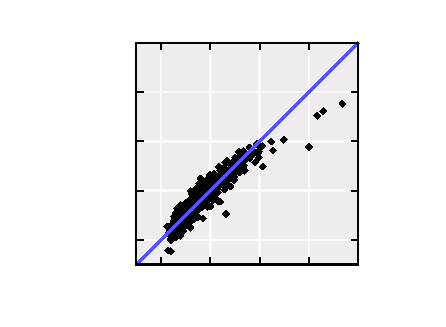
\includegraphics{gp/ms-sa-n-corr}}%
    \gplfronttext
  \end{picture}%
\endgroup

				}
				\caption{\parbox[t]{0.4\textwidth}{
					$\hat{p}^{(\m{N})} \sim p^{(\m{N})}$ \smallskip \\
					$(R^2)^{(\m{N})} = 0.861$
					}}
			\end{subfigure}
			\begin{subfigure}[t]{0.33\textwidth}
				\centerline{
					% GNUPLOT: LaTeX picture with Postscript
\begingroup
  \makeatletter
  \providecommand\color[2][]{%
    \GenericError{(gnuplot) \space\space\space\@spaces}{%
      Package color not loaded in conjunction with
      terminal option `colourtext'%
    }{See the gnuplot documentation for explanation.%
    }{Either use 'blacktext' in gnuplot or load the package
      color.sty in LaTeX.}%
    \renewcommand\color[2][]{}%
  }%
  \providecommand\includegraphics[2][]{%
    \GenericError{(gnuplot) \space\space\space\@spaces}{%
      Package graphicx or graphics not loaded%
    }{See the gnuplot documentation for explanation.%
    }{The gnuplot epslatex terminal needs graphicx.sty or graphics.sty.}%
    \renewcommand\includegraphics[2][]{}%
  }%
  \providecommand\rotatebox[2]{#2}%
  \@ifundefined{ifGPcolor}{%
    \newif\ifGPcolor
    \GPcolorfalse
  }{}%
  \@ifundefined{ifGPblacktext}{%
    \newif\ifGPblacktext
    \GPblacktexttrue
  }{}%
  % define a \g@addto@macro without @ in the name:
  \let\gplgaddtomacro\g@addto@macro
  % define empty templates for all commands taking text:
  \gdef\gplbacktext{}%
  \gdef\gplfronttext{}%
  \makeatother
  \ifGPblacktext
    % no textcolor at all
    \def\colorrgb#1{}%
    \def\colorgray#1{}%
  \else
    % gray or color?
    \ifGPcolor
      \def\colorrgb#1{\color[rgb]{#1}}%
      \def\colorgray#1{\color[gray]{#1}}%
      \expandafter\def\csname LTw\endcsname{\color{white}}%
      \expandafter\def\csname LTb\endcsname{\color{black}}%
      \expandafter\def\csname LTa\endcsname{\color{black}}%
      \expandafter\def\csname LT0\endcsname{\color[rgb]{1,0,0}}%
      \expandafter\def\csname LT1\endcsname{\color[rgb]{0,1,0}}%
      \expandafter\def\csname LT2\endcsname{\color[rgb]{0,0,1}}%
      \expandafter\def\csname LT3\endcsname{\color[rgb]{1,0,1}}%
      \expandafter\def\csname LT4\endcsname{\color[rgb]{0,1,1}}%
      \expandafter\def\csname LT5\endcsname{\color[rgb]{1,1,0}}%
      \expandafter\def\csname LT6\endcsname{\color[rgb]{0,0,0}}%
      \expandafter\def\csname LT7\endcsname{\color[rgb]{1,0.3,0}}%
      \expandafter\def\csname LT8\endcsname{\color[rgb]{0.5,0.5,0.5}}%
    \else
      % gray
      \def\colorrgb#1{\color{black}}%
      \def\colorgray#1{\color[gray]{#1}}%
      \expandafter\def\csname LTw\endcsname{\color{white}}%
      \expandafter\def\csname LTb\endcsname{\color{black}}%
      \expandafter\def\csname LTa\endcsname{\color{black}}%
      \expandafter\def\csname LT0\endcsname{\color{black}}%
      \expandafter\def\csname LT1\endcsname{\color{black}}%
      \expandafter\def\csname LT2\endcsname{\color{black}}%
      \expandafter\def\csname LT3\endcsname{\color{black}}%
      \expandafter\def\csname LT4\endcsname{\color{black}}%
      \expandafter\def\csname LT5\endcsname{\color{black}}%
      \expandafter\def\csname LT6\endcsname{\color{black}}%
      \expandafter\def\csname LT7\endcsname{\color{black}}%
      \expandafter\def\csname LT8\endcsname{\color{black}}%
    \fi
  \fi
  \setlength{\unitlength}{0.0500bp}%
  \begin{picture}(3968.00,2834.00)%
    \gplgaddtomacro\gplbacktext{%
      \csname LTb\endcsname%
      \put(886,677){\makebox(0,0)[r]{\strut{} 4}}%
      \csname LTb\endcsname%
      \put(886,1150){\makebox(0,0)[r]{\strut{} 5}}%
      \csname LTb\endcsname%
      \put(886,1623){\makebox(0,0)[r]{\strut{} 6}}%
      \csname LTb\endcsname%
      \put(886,2096){\makebox(0,0)[r]{\strut{} 7}}%
      \csname LTb\endcsname%
      \put(886,2569){\makebox(0,0)[r]{\strut{} 8}}%
      \csname LTb\endcsname%
      \put(1255,220){\makebox(0,0){\strut{} 4}}%
      \csname LTb\endcsname%
      \put(1728,220){\makebox(0,0){\strut{} 5}}%
      \csname LTb\endcsname%
      \put(2201,220){\makebox(0,0){\strut{} 6}}%
      \csname LTb\endcsname%
      \put(2674,220){\makebox(0,0){\strut{} 7}}%
      \csname LTb\endcsname%
      \put(3147,220){\makebox(0,0){\strut{} 8}}%
    }%
    \gplgaddtomacro\gplfronttext{%
      \csname LTb\endcsname%
      \put(1337,2250){\makebox(0,0)[l]{\strut{}$\overline{\m{pH}}$}}%
    }%
    \gplbacktext
    \put(0,0){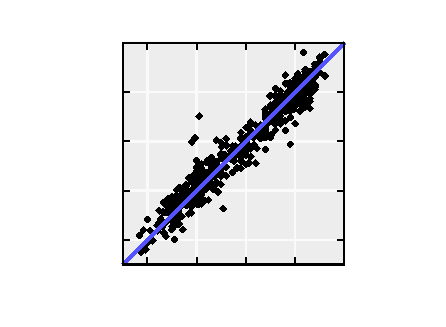
\includegraphics{gp/ms-sa-ph-corr}}%
    \gplfronttext
  \end{picture}%
\endgroup

				}
				\caption{\parbox[t]{0.43\textwidth}{
					$\widehat{\m{pH}} \sim \m{pH}$ \smallskip \\
					$(R^2)^{(\m{pH})} = 0.940$
					}}
				\label{sfig:gof-ph}
			\end{subfigure}
			\caption{Correlation diagrams plotting $\hat{y}$ on $y$ and the blue line representing the $\id$}
			\label{fig:gof}
		\end{figure*}

\section{Ergebnisse und Diskussion}
\label{sec:Ergebnisse und Diskussion}
	
	\subsection{Model Selection}
	\label{ssec:calibration}
		
	
				
	% subsection calibration

	\subsection{Bewertung der Modellwahl}
	\label{ssec:Bewertung der Modellwahl}
	    Anhand des Wertes $R^2 = 0.82$ zeigt sich, dass das gewählte Modell die Varianz in den Daten gut erklären kann.
	    Dies spiegelt auch das Korrelationsdiagramm wieder, in welchen der wahre Wert auf der x-Achse und der geschätzte Stickstoffmengenanteil $\hat{y}_i$ auf der y-Achse $y_i$ aufgetragen sind.
	    Abweichungen sind lediglich im unteren Bereich zwischen $0.0$ und $0.03$ und ab $0.3$ zu beobachten, wo der Stoffmengenanteil des Stickstoffs durch das Modell unterschätzt wird.
	    Dies lässt dich vermutlich durch die geringe Datendichte in diesen Bereichen erklären.
	    Insgesamt kann man sagen, dass die bisherigen Untersuchungen auf ausreichend gute Prognosen durch das Modell hindeuten.
		
		
	% subsection Bewertung der Modellwahl

% section Ergebnisse und Diskussion